\documentclass[11pt]{sigplanconf}

% Images
\usepackage{multicol, caption}
\usepackage{amsmath}
\usepackage{graphicx}
\graphicspath{ {images/} } % Path to images folder
\newenvironment{Figure} % Allows images to be displayed in multicols format
  {\par\medskip\noindent\minipage{\linewidth}}
  {\endminipage\par\medskip}

% Clickable URLs
\usepackage{hyperref}
\begin{document}

\special{papersize=8.5in,11in}
\setlength{\pdfpageheight}{\paperheight}
\setlength{\pdfpagewidth}{\paperwidth}

\conferenceinfo{MINES'14}{September 29, 2014, 2014, Golden, CO, USA} 
\copyrightyear{2014} 
\copyrightdata{978-1-1234-4312-1/14/12} 
\doi{543173.131664}

\titlebanner{banner above paper title}        % These are ignored unless
\preprintfooter{short description of paper}   % 'preprint' option specified.

\title{GPU-Based Parallel Finite State Machines}

\authorinfo{Kameron W. Kincade\and Ryan P. Langewisch}
           {Colorado School of Mines}
           {kkincade@mines.edu | rlangewi@mines.edu}

\maketitle

\section{Introduction}
 
A finite-state machine is used to represent an object that can exist in a limited number of states and that can change state based on a number of well-defined rules (\textit{Figure 1}). Each finite-state machine is responsible for processing various inputs (each usually represented as a string of characters) and determining if these inputs satisfy the machine's acceptance criteria, represented by ending in one of the machine's final states. To operate on an input string, the finite-state machine begins with the start state (A in \textit{Figure 1}) and processes each character one after another. The state machine's transition rules, along with the input character, dictate the next location to move to. An acceptance state (D) is commonly indicated by a double circle and represents a valid input solution that satisfies the finite-state machine's criteria.

Finite-state machines are embedded in many different types of applications, including web application computations such as lexing, parsing, translations, and media encoding/decoding. With the recent emphasis on mobile, handheld devices, the need for a computationally efficient implementation of finite-state machines is becoming more important. Parallelization is one of the obvious ways to speed up the execution of a program. However, the exclusively sequential execution of finite-state machines makes them difficult to parallelize. In this paper, we will describe some of the relevant work in the area of parallelizing finite-state machines, describe our goal and implementation progress, and then detail optimizations that we have considered adding as well as future work that could be done to extend the scope of our implementation.

\begin{Figure}
\centering
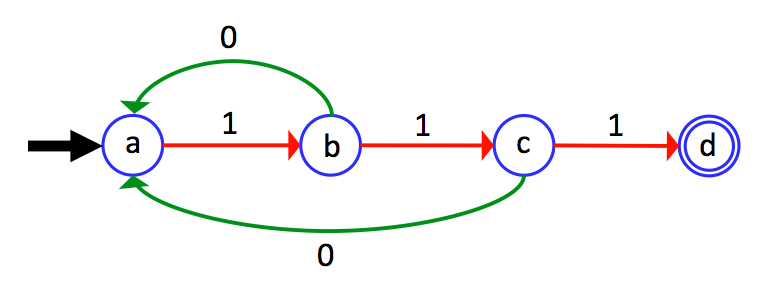
\includegraphics[width=\linewidth]{fsm_diagram.png}
\captionof{figure}{\textit{This is a simple finite-state machine example. The finite-state machine accepts input strings that have three consecutive 1's. Any other input strings are not accepted. For this example, it is assumed that our start state is state A.}}
\label{fig:Example FSM}
\end{Figure}
 
\section{Related Work}
 
The objective of parallelizing a finite-state machine is a relatively unexplored topic in computer science. To our knowledge, there are only two main publications regarding methods to parallelize finite-state machines: \textit{Data Parallel Finite-State Machines} \cite{microsoft} and \textit{Challenging the ``Embarrassingly Sequential'': Parallelizing Finite State Machine-Based Computations through Principled Speculation} \cite{william_and_mary}. The two prior publications utilize noticeably different techniques in attempts to adapt finite-state machines to work in a non-serial implementation. These two different methodologies will be described within this section.

The paper \textit{Data Parallel Finite-State Machines} \cite{microsoft} presents a parallel algorithm which performs finite-state machine computations while utilizing different kinds of data parallelism across multiple processors, as well as within a single processor. The key concept of the algorithm involves splitting the input string into distinct chunks (e.g. sub-computations on the finite-state machine) and processing the distinct chunks simultaneously. The problem with this approach is knowing the start states for each of the distinct sub-computations, as each chunk is directly influenced by the end state of the sub-computation previous to it. The authors of the paper address this data dependency by using an enumerative approach. The enumerative approach involves evaluating the sub-computation using all possible start states (i.e. enumerating over all possible start states). Once the first computation finishes, the algorithm selects the version of the enumerative computation that started from the correct start state. This process can be generalized by splitting the input string into any number of distinct chunks, with all but the first being processed in parallel.

\begin{Figure}
\centering
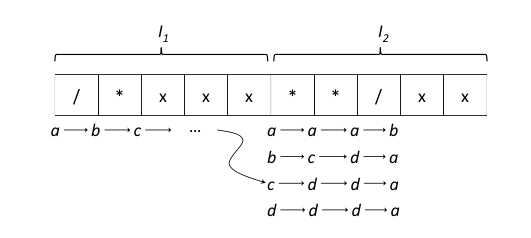
\includegraphics[width=\linewidth]{enumerative_overview.png}
\captionof{figure}{\textit{This figure is a visual representation of the enumerative approach. The first half of the input string (L1) only needs to be run once since its start state is known. However, the second half of the input string (L2) is processed by four different threads, each with a different start state (e.g. a, b, c, or d) \cite{microsoft}.}}
\label{fig:Enumerative Approach}
\end{Figure}

The main disadvantage of the enumerative approach is the amount of wasted computations being performed. This overhead is directly proportional to the amount of states within the finite-state machine. For example, a finite-state machine with n states will perform n times more computations than its corresponding serial counterpart. The paper describes different optimizations to make the enumerative computation more efficient. The main optimization relies on the assessment that many of the different enumerations of a given sub-computation converge to the same state on the same input symbol. Through dynamically utilizing this convergence, the overhead becomes proportional to the number of active states, which the authors describe as states that do not arrive from redundant (convergent) computations. This, along with other noted optimizations, offers an average of a three times speedup in exchange for the added overhead.

The other paper \textit{Challenging the ``Embarrassingly Sequential'': Parallelizing Finite State Machine-Based Computations through Principled Speculation} \cite{william_and_mary} suggests a different way of parallelizing a finite-state machine. Rather than running an enumerative computation, the authors suggest a lookback method. While still splitting the input string into multiple sub-computations, the lookback methodology attempts to provide some amount of context, using a number of ending symbols (i.e. a suffix), to help speculate the start state of a given sub-computation. The context does not necessarily provide us with the correct start state, but it can help eliminate states in which it is impossible for a given sub-computation to start with. Although this is not a new concept, the authors provide speculate as to why this approach has been rather unsuccessful in prior attempts.

\begin{Figure}
\centering
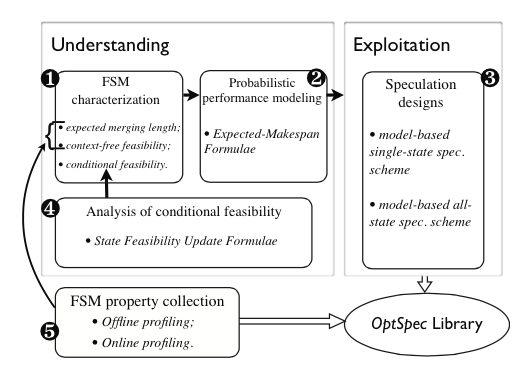
\includegraphics[width=\linewidth]{lookback_profiling_overview.png}
\captionof{figure}{\textit{This figure provides an overview of the lookback profiling technique. The process is broken down into five distinct sections, each labeled in the figure above \cite{william_and_mary}}}
\label{fig:Lookback Profiling}
\end{Figure}

The authors suggest factors, such as the number of symbols used in the lookback and the state used to begin the lookback, as just a few of the ways to possibly improve performance. They describe a collection of these factors as a speculation scheme. The main principle of their approach involves an element of profiling, by characterizing an finite-state machine and matching its properties and input to a speculation scheme that minimizes the expected make-span, which is the mean of all execution times for multiple, different length inputs. By matching a speculation scheme to a particular FSM, the concept of lookback can be utilized more efficiently, thus leading to an overall performance optimization for a given FSM and a given input string.

\section{Project Goal}

In the case of both of the fore-mentioned papers, which are the most recent and relevant work on this topic, finite-state machines were implemented in parallel, but not using GPU. It is this fact that leads us to the primary goal for our project: \textbf{Our goal is to implement deterministic finite state machines on GPU}. Additionally, we are going to focus on developing an implementation that applies all optimizations at run-time, with no prerequisite profiling. Our approach will consist of initially just getting an implementation working on GPU without any optimization, and then we will attempt to add in modular layers of optimization such as the techniques discussed in the above papers. This goal is challenging for many of the same reasons that finite-state machines are difficult to implement on CPU: the process of a finite-state machine is as sequential as a process can possibly be. Every single instruction is data dependent on the previous instruction. For this reason, it becomes an interesting problem to try and parallelize, and requires a different approach than most program optimizations using parallelization. Further interest is added to the topic due to the fact that no research has been done specifically with finite-state machines on GPU, making any progress or working implementation a contribution to the field. 

\section{Initial Approach}

In order to fully understand how to implement a parallelized version of a finite-state machine, we decided that our first step should be to decide upon the tools and hardware that should be used. As far as hardware is concerned, we currently have a good range of GPUs at our disposal. This range includes a Macbook Pro using a sixteen core NVIDIA GeForce 9400M, a Mac Pro equipped with an NVIDIA GeForce GTX 650 Ti Boost, and a GPU server provided by the Colorado School of Mines.

\begin{Figure}
\centering
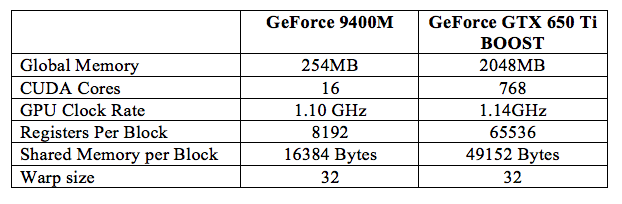
\includegraphics[width=\linewidth]{gpu_specs.png}
\captionof{figure}{\textit{The devices listed above are the three GPUs used for testing the parallelized FSM implementation. Respectively, the GPUs are components within a Macbook Pro, a Mac Pro, and a Linux server.}}
\label{fig:GPU Specifications}
\end{Figure}

Beyond hardware, the CUDA (Compute Unified Device Architecture) programming language, which is an extension of the C/C++ language developed by NVIDIA for parallel programming, was recommended as one of the easier parallel frameworks to pick up quickly. Due to the limited amount of time, a prior knowledge of the C++ language, and CUDA's compatibility with our NVIDIA GPUs, we concluded that this was the best choice of language. As a result, a large portion of our time was spent learning and understanding exactly how CUDA works. This included understanding CUDA syntax for declaring and calling kernels, how to correctly allocate and access both global and local memory, and how to collect results from each thread once it has completed its unit of work. Obviously understanding CUDA will continue to be a work in progress, but we now have a solid grasp on the framework and its underlying properties.

After deciding on a language and compatible hardware, our next step was constructing a simple, serial implementation of a finite-state machine to help us determine the the best way to represent the machine in a data structure. Our first approach was representing the finite-state machine through the use of two C++ maps, entitled \textit{fsm} and \textit{stateTransitions}. The \textit{fsm} map is responsible for mapping a state to its corresponding transition table (i.e. \textit{stateTransitions}), which is in turn responsible for mapping an input character to the next state of the finite-state machine. Therefore, determining the next state of the finite-state machine is as simple as accessing \textit{fsm[currentState][inputSymbol]}. 

With a working serial version implemented, our next goal was to implement a version of a finite-state machine that would run serially on each thread through the use of a CUDA kernel. In essence, each thread would run the exact same input on the exact same finite-state machine in order to solidify our understanding of how a CUDA application works. This seemed like a straightforward process, but the quick realization that CUDA has no support for the C++ \textit{stl} library made us rethink the whole structure of our finite-state machine. Without the use of maps, we were forced to implement a version that utilized arrays to represent our finite-state machine within memory. This new representation was structured using a two dimensional array (\textit{Figure 5}). Each row in the array represents a state in the finite-state machine, and each column corresponds to an input symbol. The resulting elements of the array represent the resulting states given a start state and an input symbol. Any finite-state machine can be converted to this format by simply indexing its states from zero and also indexing the input symbols from zero.

\begin{Figure}
\centering
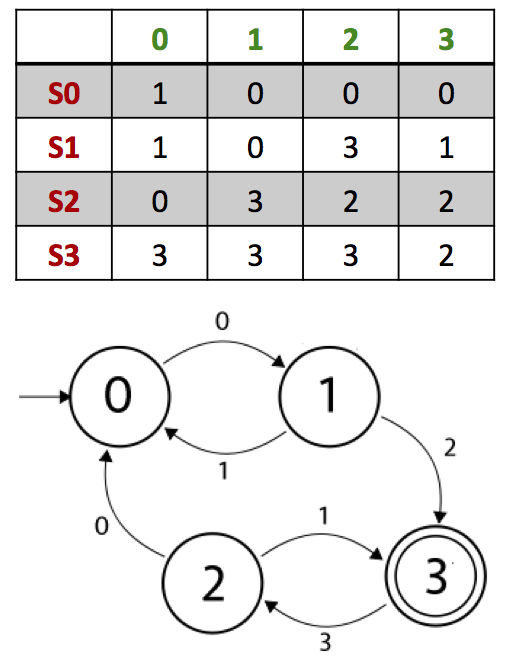
\includegraphics[width=\linewidth]{fsm_storage.png}
\captionof{figure}{\textit{The FSM is stored in a two-dimensional array where the rows represents states and the columns represent input symbols (both indexed from zero). The elements of the array are then the resulting state from the resulting row (start state) and column (input symbol).}}
\label{fig:CPU vs. GPU}
\end{Figure}

Our newly devised two-dimensional array representing our finite-state machine needed to be stored in global memory, in order for every thread to have access to it. Since all threads could reference the finite-state machine in memory, each thread required only a start state and an input string in order to run the finite-state machine and compute the corresponding end state. At this point, we essentially had a serial implementation of a finite state machine that ran on GPU. This was a good milestone in the learning process of parallel programming using CUDA, but to make the implementation worthwhile at all, we needed to apply GPU-specific optimizations in order to provide any advantage over the serial CPU implementation.

\section{Enumerative Implementation}

The primary technique that we used to improve the performance of finite-state machines on GPU was the enumerative approach, as described in the section on related work. This is the piece of our implementation that actually branches the problem into parallel executions. The basic idea is that the input string is split into a number of equal chunks determined by some predefined constant value. The first chunk, which represents the beginning of the input string, will be run on the first thread, and its result is guaranteed to be useful since it would have been the first portion of the string to be executed even if the finite-state machine was run serially. Instead of waiting for the first chunk of the string to complete to start the next chunk, we will run the second chunk in parallel using every possible start state. When the first chunk finishes, the host program will use the actual result state to determine which of the ``prediction chunks'' computed from the correct start state, and jump forward to that result. Depending on the number of chunks that were run simultaneously, the host program may be able to repeat this ``result stitching'' process many times during each iteration. 

To implement this approach, we needed to create an algorithm that could properly assign inputs to every CUDA thread, and then collect the results and piece them together accurately. The following describes our approach as outlined in \textit{Figure 6}. 

We first initialize all of the necessary variables and data structures on the host device. This includes the finite-state machine, stored as a two dimensional array, as well as various control variables and arrays for copying input to the CUDA device. For testing purposes, we used a small hard-coded finite state machine, and then used a function to generate a long input string consisting of randomly selected input symbols from the finite-state machine's alphabet. Once the data structures are in place, we allocate memory on the CUDA device in preparation for the memory copying that will take place in the main algorithm loop. We also go ahead and copy the finite-state machine into the device memory since it remains constant throughout the entire execution. Originally, we were just storing the finite-state machine in the standard global memory. This worked, but was a temporary solution as we knew that global memory did not provide fast access times, and our finite-state machine is accessed more than anything else in the implementation. We ended up converting the finite-state machine to be store in CUDA texture memory. 

\begin{Figure}
\centering
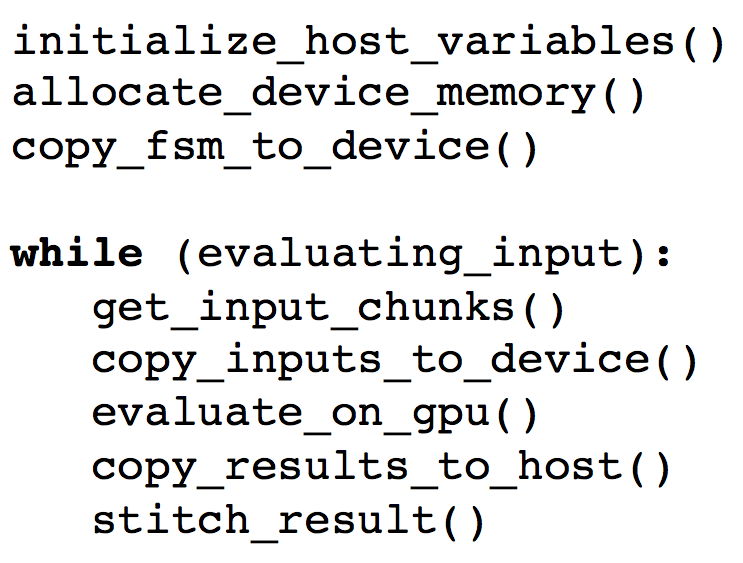
\includegraphics[width=\linewidth]{algorithm.png}
\captionof{figure}{\textit{An overview of the algorithm for parallelizing the FSM is shown here.}}
\label{fig:Algorithm}
\end{Figure}

Similar to constant memory, texture memory is read-only, but it provides an improvement in performance in cases where reads have certain access patterns \cite{textures}. After implementing the texture memory and comparing it to the previous global implementation, we found that the texture memory did improve performance, but not by a significant amount. While we did not spend much time analyzing what might have caused the lack of drastic improvement, we suspect that the finite-state machine may have not had the kind of access pattern that draws a large benefit from texture memory. For the additional arrays that were used for input and results, we added the optimization of using CUDA pitched arrays that aligns arrays in memory to allow for more effective memory coalescing.

At this point in the algorithm, everything is in place to enter the main execution loop. This loop is going to continue as long as there is still input left to be processed. The first step in this loop is generate the chunks of input that are going to be assigned to each individual thread. This consists of another loop that continues until an input has been assigned to every thread, or there is no more input remaining. Our original implementation of this step involved loading an input chunk into an array for every thread, with a one-to-one relationship. We found that this was actually inefficient due to the fact that for every sequence of threads equal to the number of states, the input chunk is identical; only the start state was varying. Instead of storing and copying so many identical inputs to the CUDA device, we changed it to only store one of each input chunk, and then used simple modulus logic based on the thread ID to retrieve the correct input during the kernel execution.

Once the input chunks have been selected, the entire input array needs to be copied into the CUDA device's memory. As will be discussed in our results section, this step proves to be a large source of overhead in our implementation. Once the input is on the device, we make the kernel call that initiates the execution of all of the threads on the GPU. Each thread uses its unique ID to access its assigned input, and then execute it from the given start state. Initially, we also copied an array of start states to the device, but we later saw that as an opportunity for optimization. Since the start states cycle in a deterministic fashion as all the different start states are used, we can again use the thread ID with some modulus logic to compute the start state without needing to pass values between the host and device. Once the input chunk has been evaluated by the thread, it copies the result into the corresponding index of a results array in global CUDA memory.

Once all threads have finished computing their results, the results array is copied back to the host device. The host is then responsible for stitching together all of the precomputed results according to the actual results. Due to the start states being indexed from zero and the enumeration of start states cycling over the same indices, each result tells us exactly what the offset is to the next desired result. Once the current state has been updated based on all of the stitched results, the entire execution loop repeats again. Once all of the input has been processed, the current state variable will hold the final state.

\section{Optimizations}

At this point in our implementation, there is no benefit from running the finite-state machine on a GPU (it is currently being ran serially), and the additional overhead of the parallel architecture actually makes it even less desirable. In order to make the GPU implementation notable at all, we need to employ strategies to specifically utilize the additional cores that are available within GPU to maximize the parallelization. 

Our first planned optimization it to implement a simple enumerative approach. This is going to be the primary technique for actually branching the problem into parallel executions. The basic idea is that that the input string is split into a number of equal chunks determined by some predefined constant value. The first chunk, which represents the beginning of the input string, will be run on the first thread, and its result is guaranteed to be useful since it would have been the first portion of the string to be executed even if the finite-state machine was run serially. But instead of waiting for the first chunk of the string to complete to start the next chunk, we are going to run the second chunk in parallel using a guess for what the initial state should be. When the first chunk finishes, the host program will use the actual result state to determine which of the ``prediction chunks'' was computing from the matching start state. This obviously leads to a lot of computed results that are left unused, but that is an advantage that comes with using GPU. Since so many threads can be run independently, we might as well be computing something on each thread rather than leaving a number of them idle. 

This will then become an iterative process: the host device first deploys the current chunk onto a GPU thread. It then deploys a number of prediction chunks that will then run in parallel with the current chunk. Once all threads complete, the host device will piece together the results based on the current chunk's final state, and determine the new current chunk. This is repeated until the entire input string is exhausted. While the core idea of this optimization technique is fairly straightforward, there are a lot of parameters that can be tweaked to affect its impact on performance. For example, the chunk size is going to have an impact on the ratio of running time on the CUDA device to the amount of overhead that the host device needs to spend deploying new threads. In addition, there are some decisions to be made about which prediction chunks should be used. 

One approach is to apply a breadth-first search to determine which chunks are deployed first. This means the second chunk is going to be deployed along with every possible start state before any threads are deployed with the third chunk of the input string. This is useful because if all the possible start states are considered for the the second chunk, the correct state is guaranteed to have been evaluated by the time the first chunk finishes. The other extreme is if we apply a depth-first search for our chunk selection strategy. This would mean that we only consider one start state for every chunk in the string, allowing many sequential chunks in the string to be run at the same time. This approach would actually be extremely ineffective, because if any of the single guessed states for a given chunk is wrong, all following chunk computations are useless because we need to recompute the chunk that was miscalculated. In other words, a strictly depth-first approach requires us to exactly guess correctly to reap any computational benefit. But a hybrid approach between breadth-first and depth-first could prove to be effective if we can find a balance between maintaining a high probability of having the next chunk result precomputed, while still having the chance of multiple chunk completion within a single kernel call.

This leads us to the topic of attempting to trim down the start states that are considered for each chunk. If we can determine that a certain start state is unreachable for that specific chunk, we can exclude it, allowing us to maximize the effectiveness of the chunks that are run during each iteration. This can be approached using the lookback technique described in one of the papers of previous work. Instead of simply running an instance of the chunk for every start state, the algorithm will also look at a certain number of input symbols before the chunk in attempt to eliminate some start states from the search space. In the paper that implemented the lookback technique, there was significant profiling that was applied before the actual parallel finite-state machine implementation was run. As stated in our goal for the project, we are trying to focus on optimizations that can be applied at runtime, without any profiling in advance. This is going to make implementing lookback slightly more challenging, as any data about what states are possible needs to be generated as part of the overall execution time.

One approach to this might be to apply some sort of dynamic learning algorithm that gathers more information about how to filter states with each iteration of chunks that is run by the finite-state machine. At the very least, a very simple implementation could be added that at least rules out states based on a small lookback. For example, if the input symbol before the chunk is a zero, we can immediately rule out any state that does not have a transition of zero moving into it. This can be applied a variable amount of steps back in the input string, which introduces another parameter to be considered. The larger the lookback, the more states that can be eliminated from the search space, freeing threads to run computations that have more potential of use. The drawback is that the overhead on the host device also increases with a larger lookback. It is another balancing act to find the most effective strategy, and the ``right answer'' is dependent on a large amount of factors including, but not limited to: the number of states in the finite-state machine, the number of different input symbols, and the current chunking strategy that is being used (the balance between breadth-first and depth-first selection of prediction chunks).

As mentioned before, our current implementation places the finite-state machine data structure into the global memory of CUDA so that it can be accessed by all of the individual threads that are running. This works fine as a preliminary approach, but global memory happens to be the slowest memory strategy in CUDA. Another optimization that could be made is to transition the finite-state machine into shared memory to allow for more efficient data accesses. The problem presented by finite-state machines has the advantage of not needing to write any data to shared memory; the finite-state machine remains constant throughout the entire run. This means that we don't need to worry about any problems caused by data racing or other dependencies in shared memory. That said, memory accesses to the finite-state machine make up the majority of the computation that happens within the CUDA kernel, and therefore any optimization to the data accesses will have its benefit multiplied significantly in the context of the entire execution.

\section{Results}

To test the parallel implementation, two particular test configurations were used. The first analyzed the impact the number of threads had on the finite-state machine's run time. The second analyzed the GPU implementation's performance versus the CPU serial version. The second test utilizes three different finite-state machines (one with 4 states, one with 16 states, and one with 64 states) along with three varying input sizes (500 million, 1 billion, and 2 billion). The input sizes are noted as S, M and L, denoting small, medium, and large respectively. The graphs refer to these different test names as a combination of the number of states and their input size. For example, 64M refers to the 64 state finite-state machine running the medium input of 1 billion input symbols. The results of these two tests are shown in \textit{Figure 7} and \textit{Figure 8}.

\begin{Figure}
\centering
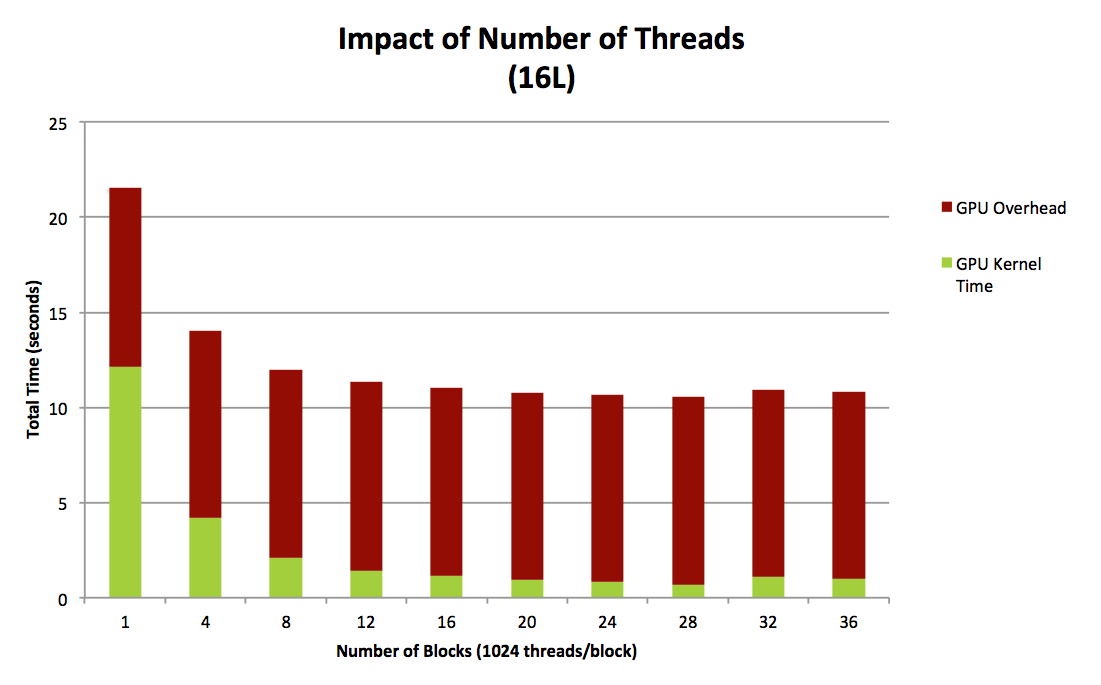
\includegraphics[width=\linewidth]{impact_of_number_of_threads.png}
\captionof{figure}{\textit{The same finite-state machine was ran using the same input but using a different number of threads. The results show that increasing the number of threads decreases the amount of GPU time. It is important to note how the overhead time stays roughly the same regardless of the number of threads being used.}}
\label{fig:Impact of Threads}
\end{Figure}

\textit{Figure 7} shows the impact of increasing the number of threads on our parallel finite-state machine implementation. As the number of useable threads increases, the GPU kernel time (i.e. the actual time spent processing input) decreases, as we would expect. The important thing to note within this graph is the consistent overhead time regardless of the number of threads being used. The overhead involved in creating input chunks and copying them to memory (the red bars of the graph) continues to be the bottleneck of the GPU implementation.

\begin{Figure}
\centering
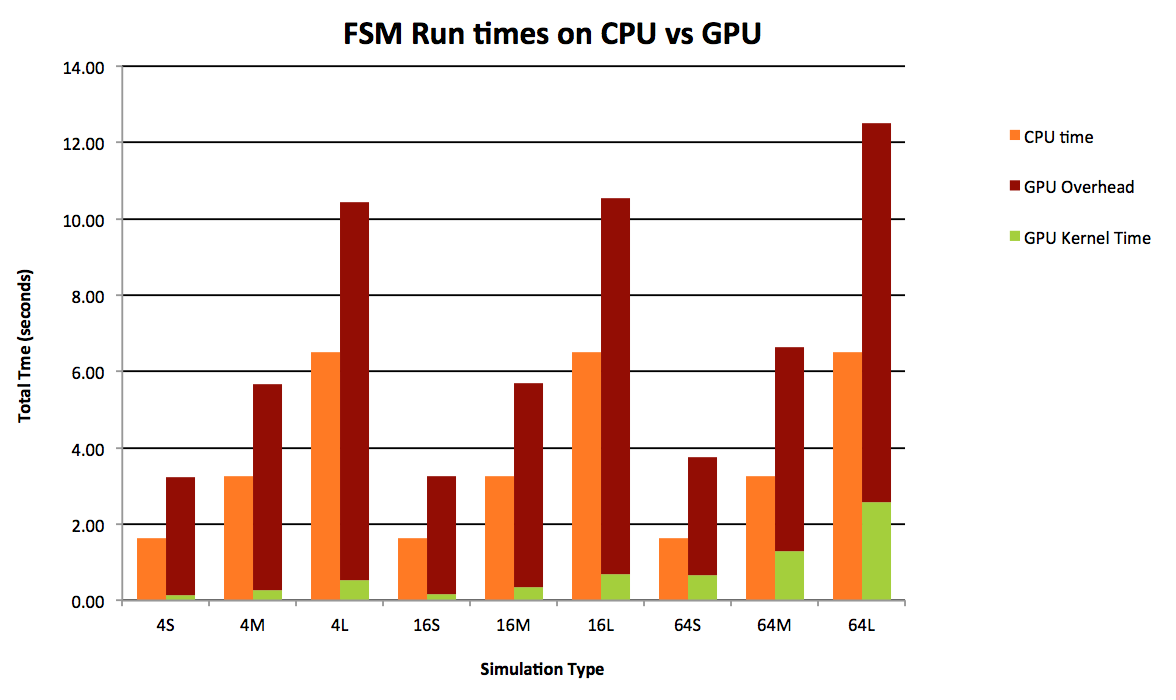
\includegraphics[width=\linewidth]{cpu_vs_gpu.png}
\captionof{figure}{\textit{The CPU time is shown in orange, the GPU overhead is shown in maroon, and the GPU kernel time is shown in green. These results show that the major bottleneck of running the GPU implementation is the overhead involved in creating the input chunks. However, the GPU kernel time is significantly lower than the CPU time.}}
\label{fig:CPU vs. GPU}
\end{Figure}

The graph shown in \textit{Figure 8} analyzes the performance of the GPU implementation against the serial CPU implementation. As evident in the graph, the total GPU time never outperforms that of the CPU. However, the GPU kernel time is significantly lower than the CPU's execution time. This once again highlights the overhead bottleneck previously mentioned. If the GPU's overhead can be decreased or eliminated, its overall performance would increase dramatically and outperform a standard serial implementation.



\section{Future Work}

As evidenced by our test results, the most important step for future work is to reduce the overhead that is necessary for the parallelized version to run. Due to the fact that memory copying is the primary cause of the inflated execution time, it may be worth looking into setups that remove this bottleneck such as an integrated GPU. We also notice that our algorithm does all of the input chunk selection serially on the host device, which is execution time where all of the GPU threads are left waiting until the host is finished. There may be opportunity for large speedup if this input selection process could be worked into the kernel call, allowing the parallelism to be utilized for a larger percentage of the algorithm's runtime.

Many other optimizations would also become possible once the host overhead is not longer a bottleneck. One example is the lookback strategy that was mentioned in the related work section. This would allow the states to be trimmed to avoid ``impossible'' configurations, and would create room for more chunks to be run during each iteration. For this specific project, we intentionally narrowed the problem scope to make it more manageable. One of the restrictions that we set for ourselves was to avoid any pre-run profiling. There is nothing about our implementation that prevents this strategy from being added, and one future extension would be to create a profiling algorithm that improves the accuracy of the decisions that the program needs to make at runtime. The scope of the problem could also be expanded to include non-deterministic finite-state machines. This would likely require a major reworking of the thread-chunking algorithm, but could allow the work be applied to other applications. Similarly, there may be different optimizations that can be made based on properties of the finite-state machine such as number of states, density of edges, and number of cycles. Due to the fact that finite-state machines can be defined with such a wide variance in properties, there are a lot of tests and specific approaches that could be applied to address different applications. Our work should lay some of the groundwork for these optimizations to be explored.


\begin{thebibliography}{9}
\softraggedright

\bibitem{microsoft} Mytkowicz, Todd. Musuvathi, Madanlal. Schulte, Wolfram. \textit{Data-Parallel Finite-State Machines}. ASPLOS. March 5, 2014.

\bibitem{william_and_mary} Zhao, Zhijia. Wu, Bo. Shen, Xipeng. \textit{Parallelizing Finite State Machine-Based Computations through Principled Speculation}. ASPLOS. March 5, 2014.

\bibitem{textures} Gupta, Nitin. \textit{Texture Memory in CUDA\: What is texture memory in CUDA Programming} \url{http://cuda-programming.blogspot.com/2013/02/texture-memory-in-cuda-what-is-texture.html}. Nov, 2012.

\end{thebibliography}


\end{document}